\documentclass{article}

\usepackage{kotex}
\usepackage{fancyhdr}
\usepackage{extramarks}
\usepackage{amsmath}
\usepackage{amsthm}
\usepackage{amsfonts}
\usepackage{amssymb}
\usepackage{tikz}
\usepackage[plain]{algorithm}
\usepackage{algpseudocode}
\usepackage{ytableau}

\usetikzlibrary{automata,positioning}

%
% Basic Document Settings
%

\topmargin=-0.45in
\evensidemargin=0in
\oddsidemargin=0in
\textwidth=6.5in
\textheight=9.0in
\headsep=0.25in

\linespread{1.1}

\pagestyle{fancy}
\lhead{\hmwkAuthorName}
\chead{\hmwkClass\ (\hmwkClassInstructor): \hmwkTitle}
\rhead{\firstxmark}
\lfoot{\lastxmark}
\cfoot{\thepage}

\renewcommand\headrulewidth{0.4pt}
\renewcommand\footrulewidth{0.4pt}

\setlength\parindent{0pt}

\newcommand\numberthis{\addtocounter{equation}{1}\tag{\theequation}}

%
% Create Problem Sections
%

\newcommand{\enterProblemHeader}[1]{
    \nobreak\extramarks{}{Problem \arabic{#1} continued on next page\ldots}\nobreak{}
    \nobreak\extramarks{Problem \arabic{#1} (continued)}{Problem \arabic{#1} continued on next page\ldots}\nobreak{}
}

\newcommand{\exitProblemHeader}[1]{
    \nobreak\extramarks{Problem \arabic{#1} (continued)}{Problem \arabic{#1} continued on next page\ldots}\nobreak{}
    \stepcounter{#1}
    \nobreak\extramarks{Problem \arabic{#1}}{}\nobreak{}
}

\setcounter{secnumdepth}{0}
\newcounter{partCounter}
\newcounter{homeworkProblemCounter}
\setcounter{homeworkProblemCounter}{1}
\nobreak\extramarks{Problem \arabic{homeworkProblemCounter}}{}\nobreak{}

%
% Homework Problem Environment
%
% This environment takes an optional argument. When given, it will adjust the
% problem counter. This is useful for when the problems given for your
% assignment aren't sequential. See the last 3 problems of this template for an
% example.
%
\newenvironment{homeworkProblem}[1][-1]{
    \ifnum#1>0
        \setcounter{homeworkProblemCounter}{#1}
    \fi
    \section{Problem \arabic{homeworkProblemCounter}}
    \setcounter{partCounter}{1}
    \enterProblemHeader{homeworkProblemCounter}
}{
    \exitProblemHeader{homeworkProblemCounter}
}

%
% Homework Details
%   - Title
%   - Due date
%   - Class
%   - Section/Time
%   - Instructor
%   - Author
%

\newcommand{\hmwkTitle}{Homework\ \#4}
\newcommand{\hmwkDueDate}{November 15, 2016}
\newcommand{\hmwkClass}{CS300}
\newcommand{\hmwkClassInstructor}{Prof. Sunghee Choi}
\newcommand{\hmwkAuthorName}{Ohjun Kwon}

%
% Title Page
%

\title{
    \vspace{2in}
    \textmd{\textbf{\hmwkClass:\ \hmwkTitle}}\\
    \normalsize\vspace{0.1in}\small{Due\ on\ \hmwkDueDate\ at 10:30am}\\
    \vspace{0.1in}\large{\textit{\hmwkClassInstructor}}
    \vspace{3in}
}

\author{\textbf{20160051 \hmwkAuthorName}}
\date{}

\renewcommand{\part}{\textbf{\large Part \Alph{partCounter}}\stepcounter{partCounter}\\}

%
% Various Helper Commands
%

% Useful for algorithms
\newcommand{\alg}[1]{\textsc{\bfseries \footnotesize #1}}

% For derivatives
\newcommand{\deriv}[1]{\frac{\mathrm{d}}{\mathrm{d}x} (#1)}

% For partial derivatives
\newcommand{\pderiv}[2]{\frac{\partial}{\partial #1} (#2)}

% Integral dx
\newcommand{\dx}{\mathrm{d}x}

% Alias for the Solution section header
\newcommand{\solution}{\textbf{\large Solution}}

% Probability commands: Expectation, Variance, Covariance, Bias
\newcommand{\E}{\mathrm{E}}
\newcommand{\Var}{\mathrm{Var}}
\newcommand{\Cov}{\mathrm{Cov}}
\newcommand{\Bias}{\mathrm{Bias}}

\begin{document}

\maketitle

\pagebreak
\begin{homeworkProblem}
    \textbf{(a)}
    $x_i$가 가질 수 있는 $h$개의 값의 후보를 $a_1, a_2, \dots, a_h$라고 하고,
    이를 모은 집합을 $A=\{a_1,a_2,\dots ,a_h\}$라고 하고,
    \begin{equation}
        \sum_{i=1}^nm_i(x_i)+\sum_{i=2}^n\phi (x_{i-1},x_i)
        \label{eq:fx}
    \end{equation}
    식~\ref{eq:fx}\를 최소로 만드는 $(x_1, x_2, \dots, x_n)$을 $L(n)$이라고 하면,
    우리가 구하고자 하는 정보를 $L(n)$이라고 나타낼 수 있을 것이다.
    그렇다면 $L(n)$은 $L(n-1)$에 $f(x)$의 값을 최소로 만드는 하나의 $x_n\in A$를 찾아 $L(n-1)$에 연장시켜주는 방식으로 생각하면 될 것이다.
    하지만, 이 방법에서는 $L(n)$이 $L(n-1)$에 하나의 숫자를 끝에 붙인 형태가 아닐 수도 있어 약간의 결점이 있다.
    예를 들면, 우리가 구한 $L(n-1)$에서 $x_{n-1}$이 $q$라고 하면 이 $q$와 마지막 $x_n$의 관계($\phi$) 중에 가장 작은 수를 $A$에서 찾게 될 것인데,
    $\phi(q,r)$ ($\forall r \in A$)의 값이 모두 커 다른 수열을 통해서 $x_n$까지 도달하는 방향으로 찾는 것이 더 작은 $f(x)$를 찾게 될 수도 있다.
    그런 상황에 대비하기 위해서 우리는 $L(n)$을 찾을 때 다른 경로를 통해서 찾을 수 있도록 잡아야 할 것이다.
    식~\ref{eq:fx}\를 최소로 만드는 $(x_1, x_2, \dots, x_{n-1}, x_n=k)$를 $L(n,k)$라고 하자.
    (단, $k\in A$). 이렇게 설정하면 최후에 $L(n)$은 $f(L(n,k))$를 최소화 하는 $L(n,k)$가 될 것이다.
    이제 각 값을 찾는 방법에 대해서 설명하자면, $L(n,k)$를 찾기 위해서 전 단계의 결과를 참조하도록 하자.
    \begin{equation}
        \min_{q\in A}\left\{ m_{n-1}(k)+\phi(q,k)\right\}
        \label{eq:qk}
    \end{equation}
    식~\ref{eq:qk}을 만족하는 $q$를 찾으면 $L(n,k)$는 $L(n-1,q)$의 맨 끝에 $k$를 붙인 것이 된다.
    \begin{figure}[!ht]
        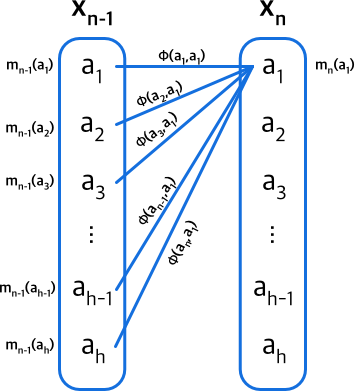
\includegraphics[height=0.3\textheight]{1a1}
        \centering
        \caption{$L(n,a_1)$을 찾는 과정}
        \label{fig:1a1}
    \end{figure}
    이것을 $h$번 하면 $L(n)$을 구할 수 있게 된다. 이는 $O(h^2)$의 시간이 걸리게 되고,
    이를 $L(1)$일 때부터 $L(n)$일 때까지 계산은 총 $n$번 하므로 총 $O(nh^2)$의 시간이 걸리게 된다.
    이를 의사코드로 나타내면 아래와 같다.
    \begin{algorithm}[!ht]
        \begin{algorithmic}[1]
            \Function{L}{$n$}
                \State $L[1\dots n,1\dots h]$ $\triangleright$ $L(n,k)$ 메모이제이션 행렬
                \State $M[1\dots h]$ $\triangleright$ $f(x)$를 저장해두는 행렬
                \For{$i\gets 1$ to $n$}
                    \For{$j\gets 1$ to $h$}
                        \If{$i=1$}
                            \State $L[i,j]\gets [a_j]$
                            \State $M[j]\gets 0$
                        \Else
                            \State $q\gets \min_{1\leq i\leq h}\left\{m_{n-1}(a_j)+\phi(a_i,a_j)\right\}$ 일 때 $i$
                            \State $L[i,j]\gets L[i-1,q]$.append$(a_j)$
                            \State $M[j]\gets M[j]+m_{n-1}(a_j)+\phi(a_q,a_j)$
                        \EndIf
                    \EndFor
                \EndFor
                \State $k\gets \min_{1\leq i\leq h}M[i]$ 일 때 $i$
                \State \Return $L[n,k]$
            \EndFunction
        \end{algorithmic}
    \end{algorithm}

    알고리즘 \alg{L}의 시간복잡도를 줄 별로 계산해보면,
    이중 for문내의 문장들은 $O(nh)$번 실행되게 될 것인데,
    10번째 줄에서 최소를 찾을 때 $O(h)$의 시간이 걸린다.
    그러므로 이중 for문을 탈출하기까지는 $O(nh^2)$의 시간이 걸리고,
    $L(n,k)$에서 $f(x)$의 최솟값을 이용하여 $L(n)$을 찾아내는 부분인 16번째 줄은 $O(h)$의 시간이 걸린다.
    그러므로 총 $O(nh^2)$의 시간복잡도를 갖는다.
    \\

    \textbf{(b)}
    $G$를 가중치가 적힌 유향그래프의 인접행렬이라고 하고,
    $path(i,k)$를 $v_i$로 끝나는 $(s_1, s_2, \dots, s_k)$의 경로라고 두자.
    그러면 $path(i,k)$는 $path(\cdot,k-1)$을 전부 검사하여 그곳에서 해당하는 $s_k$를 가진 간선이 있는지 여부를 확인하여
    만약 있으면 그 경로에 끝에 이동 할 수 있는 곳을 붙여주면 된다.
    그렇게 하면 $path(\cdot, k)$에는 원했던 답인 $s$를 거쳐 갈 수 있는 경로가 남는다.
    의사코드 \alg{Find}에는 그 중 정점의 번호가 가장 작은 곳에 도착하는 경로를 출력하도록 하였다.
    $path(\cdot,k)$에 아무런 경로가 남지 않는다면 그 경로는 갈 수 없는 경로이므로 \textbf{No-Such-Path}\를 출력하도록 하였다.
    (의사코드 \alg{Find}\를 Python 2로 구현한 실제 작동하는 코드를 첨부하였다.)
    \begin{algorithm}[!ht]
        \begin{algorithmic}[1]
            \Function{Find}{$G, s$}
                \State $path[0\dots n,0\dots k]$을 생성하고 전부 $None$으로 초기화 $\triangleright$ $path(i,k)$의 메모이제이션 행렬
                \State $path[0,0]\gets [0]$
                \For{$l\gets 1$ to $k$}
                    \For{$i\gets 0$ to $n$}
                        \If{$path[i,l-1]\neq None$}
                            \For{$j\gets 0$ to $n$}
                                \If{$G[i,j] = s_l$}
                                    \State $path[j, l]\gets path[i,l-1]$
                                    \State $path[j,l]$.append$(j)$
                                \EndIf
                            \EndFor
                        \EndIf
                    \EndFor
                \EndFor
                \For{$i\gets 0$ to $n$}
                    \If{$path[i,k]\neq None$}
                        \State \Return $path[i,k]$
                    \EndIf
                \EndFor
                \State \Return ``No-Such-Path''
            \EndFunction
        \end{algorithmic}
    \end{algorithm}
\end{homeworkProblem}
\pagebreak
\begin{homeworkProblem}
    $G$를 그래프의 인접리스트라고 하면,
    인접한 정점끼리의 색이 겹치지 않도록 주변의 모든 정점의 색을 판단한 후 사용되지 않은 색을 칠하는 방식으로 하면 된다.
    다만, 색을 칠할 때 최대한 사용했던 색을 사용하도록 하기 위해서 색에 번호를 부여한 후 작은 번호부터 차례로 체크하도록 하였다.
    주변의 정점끼리만 비교해서 최소의 색을 사용하도록 하면 이가 전체의 해가 된다.
    그래프 $G$를 주어진 조건에 맞게 색칠하는 알고리즘은 \alg{Color}와 같이 짤 수 있다.
    (의사코드 \alg{Color}를 Python 2로 구현한 예제는 뒤에 첨부되어 있다.)
    \begin{algorithm}[!ht]
        \begin{algorithmic}[1]
            \Function{Color}{$G$}
                \State $A[0\dots |V|]$을 생성하고 전부 $0$으로 초기화한다. $\triangleright$ $A[i]$: $i$번째 정점에 칠해진 색
                \For{$i\gets 0$ to $|V|$}
                    \State $used[0\dots |V|+1]$을 생성하고 전부 \textbf{False}로 초기화한다. $\triangleright$ $used[i]$: 색 $i$가 칠해진 여부
                    \State $used[0]\gets$ \textbf{True} $\triangleright$ 색을 $1$부터 시작하게 하기 위해
                    \For{$j\in G[i]$}
                        \State $used[A[j]]\gets$ \textbf{True}
                    \EndFor
                    \For{$j\gets 0$ to $|V|+1$}
                        \If{not $used[j]$}
                            \State $A[i]\gets j$
                            \State \textbf{Break}
                        \EndIf
                    \EndFor
                \EndFor
                \State \Return $A$
            \EndFunction
        \end{algorithmic}
    \end{algorithm}

    알고리즘 \alg{Color}의 시간복잡도를 계산해보자.
    첫 번째 for문 내부를 보면 for문이 하나 더 있는데 전부 펼쳐져 있기 때문에
    for문 내부의 문장들은 $O(|V|)$번 실행되게 된다.
    그러므로 전체적으로는 $O(V^2)$의 시간복잡도를 가지게 된다.
\end{homeworkProblem}
\end{document}
